\chapter{Caminos de operaci�n}

\textbf{\textit{En este cap�tulo comentaremos los diagramas de secuencia que
seguir�an las comunicaciones entre los componentes para tener una idea general
del sistema de modo visual.}}



\section{Autentificaci�n}

Para la autentificaci�n con \dplc y verificaci�n de los datos firmados de �ste,
hace falta previamente conocer su clave p�blica.
%TODO: que pasa al recibir datos firmados/encriptados con una clave que no
%conocemos?

Con tal de acceder un cliente (\dpld) a un nodo (\dplc), �ste debe primero
registrarse envi�ndole la clave y password de SSH \textbf{encriptados} con la
clave p�blica de \dplc (para evitar que informaci�n sensible sea capturada).

Para ello, hay dos primitivas de autentificaci�n, una que hace una
autentificaci�n con respuesta (destinada a un solo nodo), y otra que hace la
autentificaci�n con todo el grupo multicast, pero que no da ning�n resultado.

El proceso completo es el que se muestra en la figura \ref{fig:act_-_auth}.

\begin{figure}[h]
	\centering
	\includegraphics[scale=1.0]{act_-_auth.eps}
	\caption{Proceso de autentificaci�n}
	\label{fig:act_-_auth}
\end{figure}



\section{Listado de nodos}

El comando que lanzar�a esta operaci�n seria \texttt{ls /plfs/nodes/}, y el
diagrama de sus operaciones es el que se muestra en la figura
\ref{fig:act_-_ls_nodes}.

\begin{figure}[h]
	\centering
	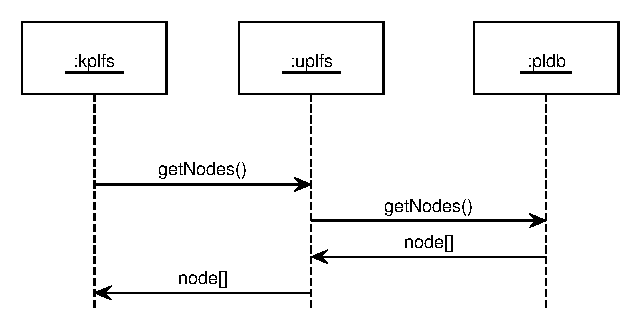
\includegraphics[scale=1.0]{act_-_ls_nodes.eps}
	\caption{Listado de nodos}
	\label{fig:act_-_ls_nodes}
\end{figure}



\section{Listado de slices}

El comando que lanzar�a esta operaci�n seria \texttt{ls /plfs/slices/}, y el
diagrama de sus operaciones es el que se muestra en la figura
\ref{fig:act_-_ls_slices}.

\begin{figure}[h]
	\centering
	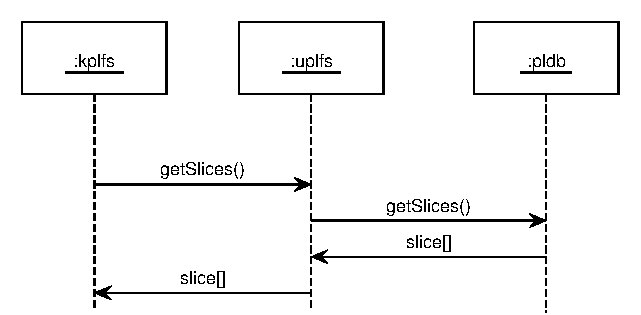
\includegraphics[scale=1.0]{act_-_ls_slices.eps}
	\caption{Listado de slices}
	\label{fig:act_-_ls_slices}
\end{figure}



\section{Listado de ficheros compartidos}

El comando que lanzar�a esta operaci�n ser�a \texttt{ls
/plfs/slices/\textless{}slice\textgreater/shared/}, y el diagrama de sus
operaciones es el que se muestra en la figura \ref{fig:act_-_ls_shared}.

\begin{figure}[h]
	\centering
	\includegraphics[scale=1.0]{act_-_ls_shared.eps}
	\caption{Listado de ficheros compartidos}
	\label{fig:act_-_ls_shared}
\end{figure}



\section{Listado de nodos de un slice}

El comando que lanzar�a esta operaci�n ser�a \texttt{ls
/plfs/slices/\textless{}slice\textgreater/nodes/}, y el diagrama de sus
operaciones es el que se muestra en la figura \ref{fig:act_-_ls_slice_nodes}.

\begin{figure}[h]
	\centering
	\includegraphics[scale=1.0]{act_-_ls_slice_nodes.eps}
	\caption{Listado de nodos de un slice}
	\label{fig:act_-_ls_slice_nodes}
\end{figure}



\section{Listado de ficheros no compartidos}

El comando que lanzar�a esta operaci�n ser�a \texttt{ls
/plfs/slices/\textless{}slice\textgreater/nodes/\textless{}node\textgreater/unshared/},
y el diagrama de sus operaciones es el que se muestra en la figura
\ref{fig:act_-_ls_unshared}.

\begin{figure}[h]
	\centering
	\includegraphics[scale=1.0]{act_-_ls_unshared.eps}
	\caption{Listado de ficheros no compartidos}
	\label{fig:act_-_ls_unshared}
\end{figure}



\section{Obtenci�n de un fichero}

El comando que lanzar�a esta operaci�n ser�a, por ejemplo, un \texttt{cat} de
un fichero, ya fuera en \texttt{shared} o \texttt{unshared}, y el diagrama de
sus operaciones es el que se muestra en la figura \ref{fig:act_-_get}.

\begin{figure}[h]
	\centering
	\includegraphics[scale=1.0]{act_-_get.eps}
	\caption{Obtenci�n de un fichero}
	\label{fig:act_-_get}
\end{figure}



\section{Despliegue}

% TODO: desplegar el soft de despliegue si no esta presente y es un nuevo
% nodo?

El comando que lanzar�a esta operaci�n ser�a, por ejemplo, un \texttt{cp} de
un fichero, ya fuera a \texttt{shared} a \texttt{unshared}, y el diagrama de
sus operaciones es el que se muestra en la figura \ref{fig:act_-_put}.

\begin{figure}[h]
	\centering
	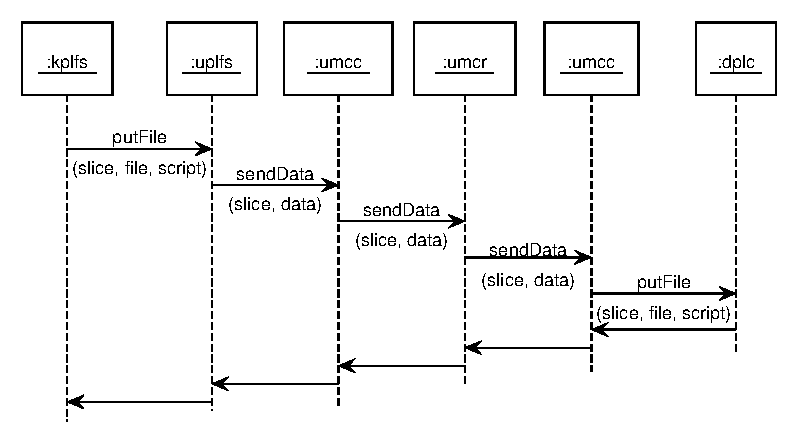
\includegraphics[scale=1.0]{act_-_put.eps}
	\caption{Despliegue}
	\label{fig:act_-_put}
\end{figure}



\section{Adici�n de un nodo a un grupo}

�sta operaci�n se llevar�a a cabo al crear una nueva m�quina virtual en un
nodo donde ya este corriendo \dplc, y el diagrama de sus operaciones es el que
se muestra en la figura \ref{fig:act_-_join}.

\begin{figure}[h]
	\centering
	\includegraphics[scale=1.0]{act_-_join.eps}
	\caption{Adici�n de un nodo a un grupo}
	\label{fig:act_-_join}
\end{figure}



\section{Eliminaci�n de un nodo de un grupo}

�sta operaci�n se llevar�a a cabo al eliminar una m�quina virtual de un nodo
donde ya este corriendo \dplc, y el diagrama de sus operaciones es el que se
muestra en la figura \ref{fig:act_-_delete}.

\begin{figure}[h]
	\centering
	\includegraphics[scale=1.0]{act_-_delete.eps}
	\caption{Eliminaci�n de un nodo de un grupo}
	\label{fig:act_-_delete}
\end{figure}
